\def\mySecNum{9.1}
\mySection{\mySecNum~Put-call parity}
%-------------- start slide -------------------------------%{{{ 1
\begin{frame}[fragile]
\begin{center}
	How does one value the right to back away from a commitment?
	\bigskip

	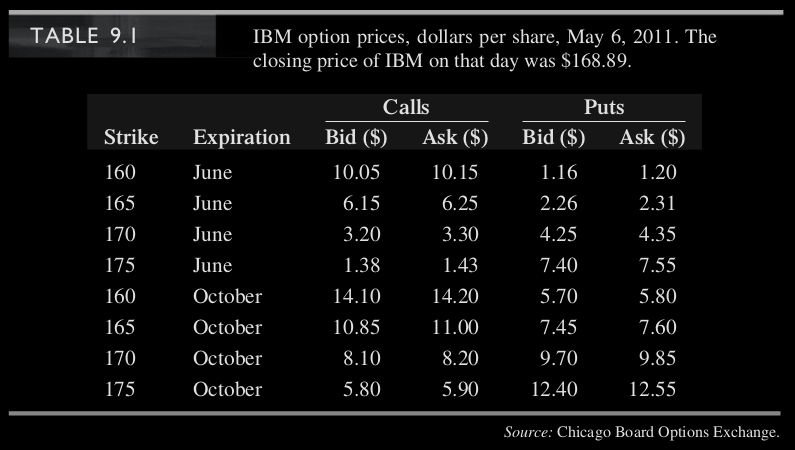
\includegraphics[scale=0.25]{figs/Table-9-1.png}
\end{center}
\end{frame}
%-------------- end slide -------------------------------%}}}
%-------------- start slide -------------------------------%{{{ 1
\begin{frame}[fragile,t]
	\begin{itemize}
		\item What determines the difference between put and call prices at a given strike?
		\item How would the premiums change if these options were European rather than American?
		\item It appears that, for a given strike, the October options are more expensive than the June options. Is this necessarily true?
		\item Do call premiums always decrease as the strike price increases? Do put premiums always increase as the strike price increases?
		\item Both call and put premiums change by less than the change in the strike price. Does this always happen?
	\end{itemize}
\end{frame}
%-------------- end slide -------------------------------%}}}
%-------------- start slide -------------------------------%{{{ 1
\begin{frame}[fragile,t]
	\frametitle{European options}

	\begin{align*}
		C(K,T) - P(K,T) & = \text{PV}_{0,T} \left(F_{0,T}-K\right) \\
                    & = e^{-rT}\left(F_{0,T}-K\right)
	\end{align*}

	\pause
	\bigskip
	\begin{center}
		Buying a call and selling a put \\
		with the strike both equal to the forward price (i.e., $K=F_{0,T}$)\\
		creates a synthetic forward contract \\
		and hence must have a zero price.

		\pause
		\bigskip
		\mySeparateLine
		\bigskip

		Parity generally fails for American options!
	\end{center}
\end{frame}
%-------------- end slide -------------------------------%}}}
%-------------- start slide -------------------------------%{{{ 1
\begin{frame}[fragile,t]
	\frametitle{Parity for stocks}
	\begin{align*}
		C(K,T) = P(K,T) + \left(S_0-\text{PV}_{0,T}(\text{Div})\right) - e^{-rT} K
	\end{align*}
\end{frame}
%-------------- end slide -------------------------------%}}}
%-------------- start slide -------------------------------%{{{ 1
\begin{frame}[fragile,t]
	\begin{myexample}
		\label{Eg:9-1}
		Suppose that the price of a non-dividend-paying stock is \$40, the continuously compounded
		interest rate is 8\%, and options have 3 months to expiration. If a 40-strike European call
		sells for \$2.78, find the price for a 40-strike European put sells.
	\end{myexample}
	\bigskip
	\pause
	\begin{mysol}
		Let the price for put be $y$. Then
		\begin{align*}
			\$2.78 = y + \$40 - \$40e^{−0.08\times0.25}
		\end{align*}
		Hence,
		\begin{align*}
			y = \$1.99.
		\end{align*}
		\myEnd
	\end{mysol}
\end{frame}
%-------------- end slide -------------------------------%}}}
%-------------- start slide -------------------------------%{{{ 1
\begin{frame}[fragile,t]
	\begin{center}
		Why is a call more expensive than a put?

		\pause
		\bigskip
		\mySeparateLine
		\bigskip

		When $S_0=K$ and $\text{Div}=0$, then
		\begin{align*}
			C(K,T)-P(K,T) = K \left(1-e^{-rT}\right)
		\end{align*}
		\bigskip

		\pause
		The difference of a call and put is\\
		the \textcolor{cyan}{time value of money}.
	\end{center}
\end{frame}
%-------------- end slide -------------------------------%}}}
%-------------- start slide -------------------------------%{{{ 1
\begin{frame}[fragile,t]
	\begin{myexample}
Make the same assumptions as in Example \myref{Eg:9-1}, except suppose that the
stock pays a \$5 dividend just before expiration. If the price of the European call is \$0.74, what
would be the price of the European put?
	\end{myexample}
	\bigskip
	\pause
	\begin{mysol}
		Let the price for put be $y$. Then
		\begin{align*}
			\$0.74 = y + \left(\$40 - \$5 e^{-0.08 \times 0.25}\right) - \$40e^{−0.08\times0.25}
		\end{align*}
		Hence,
		\begin{align*}
			y = \$4.85.
		\end{align*}
		\myEnd
	\end{mysol}
\end{frame}
%-------------- end slide -------------------------------%}}}
%-------------- start slide -------------------------------%{{{ 1
\begin{frame}[fragile,t]
	\frametitle{Synthetic securities}
	\begin{align*}
		C(K,T) = P(K,T) + \left(S_0-\text{PV}_{0,T}(\text{Div})\right) - e^{-rT} K
	\end{align*}
	\mySeparateLine

	\begin{itemize}
		\item \textcolor{magenta}{Synthetic stock}
			\begin{align*}
				\textcolor{magenta}{S_0} = C(K,T) - P(K,T) + \text{PV}_{0,T}\left(\text{Div}\right) + e^{-rT} K
			\end{align*}
	\end{itemize}
\end{frame}
%-------------- end slide -------------------------------%}}}
%-------------- start slide -------------------------------%{{{ 1
\begin{frame}[fragile,t]
	\begin{align*}
		C(K,T) = P(K,T) + \left(S_0-\text{PV}_{0,T}(\text{Div})\right) - e^{-rT} K
	\end{align*}
	\mySeparateLine

	\begin{itemize}
		\item \textcolor{magenta}{Synthetic Treasury bill (T-bill)}
			\begin{align*}
				\underbrace{S_0 - C(K,T) + P(K,T)}_{\text{a \textcolor{cyan}{\bf conversion} }} = \text{PV}_{0,T}\left(\text{Div}\right) + e^{-rT} K
			\end{align*}
			\bigskip
			\bigskip

		\item[] Motivation:
		\item[] A hedged position that has no risk but requires investment.
		\item[]  T-bills are taxed differently than stocks.
	\end{itemize}
\end{frame}
%-------------- end slide -------------------------------%}}}
%-------------- start slide -------------------------------%{{{ 1
\begin{frame}[fragile,t]
	\frametitle{Synthetic securities}
	\begin{align*}
		C(K,T) = P(K,T) + \left(S_0-\text{PV}_{0,T}(\text{Div})\right) - e^{-rT} K
	\end{align*}
	\mySeparateLine

	\begin{itemize}
		\item \textcolor{magenta}{Synthetic options}
			\bigskip
			\begin{align*}
				\textcolor{magenta}{C(K,T)} = P(K,T) + \left(S_0-\text{PV}_{0,T}(\text{Div})\right) - e^{-rT} K
			\end{align*}
			\begin{align*}
				\textcolor{magenta}{P(K,T)} = C(K,T) - \left(S_0-\text{PV}_{0,T}(\text{Div})\right) + e^{-rT} K
			\end{align*}
	\end{itemize}
\end{frame}
%-------------- end slide -------------------------------%}}}
